%!TEX root = ../thesis.tex
%%--------------------------------------------------------------------------
%% ADOCK
%%--------------------------------------------------------------------------

%% REMEMBER:
%% - section
% \section{Section Title}
% \label{sec:section_title}
%
% - subsection
% \subsection{Subsection Title}
% \label{sub:sub_title}
%
% - paragraph
% \subparagraph{Paragraph Title}
% \label{subp:subp_title}


% --------------------------------------------------------------------------- %
% ---------------------------------- ADOCK ---------------------------------- %
% --------------------------------------------------------------------------- %


\section{Our Solution, aDock}
\label{sec:adock_intro}
The lack of a uniform and standardized test environment for cloud systems brought us to develop aDock.\\
aDock is a suite of tools that lets the final user deploy a complete OpenStack system; run simulations against it; collect output data and view results on a friendly user interface.\\
We chose OpenStack as our reference cloud computing software platform, because it is open-source and because it is continuously evolving to keep up with the latest cloud standards.\\
Our intended users are OpenStack developers who need to run their code in a fully functional environment, and researchers who want to try their algorithms (e.g. about virtual machine placement or consolidation) on a complete cloud system to test out their behavior.

\section{Requirements}
\label{sec:adock_reqs}
In this section, we will identify both the functional and non-functional requirements for aDock. Functional requirements lead us to define the general architecture of the system proposed, aDock, which we show in figure \ref{fig:adock_high_arch}. Non-functional requirements lead us to precise choices in technologies used to develop the system.

\subsection{Functional Requirements}
\label{sub:func_req}

\paragraph{FR1}\label{p:fr1} \emph{aDock should provide tools to deploy a complete environment.} \hfill \\
A user should be able to start and update OpenStack's nodes with a single command and to decide which services will be installed and started on each node and their internal configuration using a configuration file.

\paragraph{FR2}\label{p:fr2} \emph{aDock should provide a tool to run simulations.} \hfill \\
If the user puts his/her code into OpenStack he/she probably will need to run simulations and examine how the new piece of code behaviors in interacting within the rest of the system. Simulations should be configurable according to the user needs and repeatable.

\paragraph{FR3}\label{p:fr3} \emph{aDock should persistently store the simulations' output.} \hfill \\
Once a simulation has been run, it could be interesting to store its outputs in terms of generic metrics about the system, such as the average number of compute nodes active during the simulation, the average number of virtual CPUs used, and so on.

\paragraph{FR4}\label{p:fr4} \emph{aDock should provide a user interface.} \hfill \\
Simulation results should be displayed to the user in a friendly manner, using charts to give the user a glimpse of the current situation. Data representation should also be given in real-time.

\subsection{aDock Modules}
\label{sub:adock_modules}

FakeStack (see section \ref{sec:fakestack}) is the aDock module which provides the user with the tools specified in requirement $1$ (see paragraph \ref{p:fr1}). FakeStack provides the concept of ``node'' which, in its depth, is an Ubuntu based Docker container, shipped with OpenStack services dependencies. Starting a node is as easy as \code{\$ run\_node}. A node can be configured by means of a simple configuration file. Nodes are of two types, \textit{controllers} and \textit{computes}. Controller nodes are different from compute ones because they are shipped with \textit{MySQL} and \textit{RabbitMQ} installations.

Oscard (see section \ref{sec:oscard}) is the simulation tool that satisfies requirement $1$ and $2$ (see paragraphs \ref{p:fr2} and \ref{p:fr3}). Oscard is the aDock module which takes care of running repeatable and configurable simulations against an OpenStack system and to store outputs persistently. This module, by default, stores the aggregates of a simulation into a Firebase\footnote{\url{https://www.firebase.com/}} backend. In our case, the backend is called Bifrost (see section \ref{sec:others}).

Although Firebase provides an interactive user interface, data is displayed as \textit{JSON} and is, therefore, not easily understandable and browseable. Polyphemus (see section \ref{sec:others}) is the aDock module that takes care of displaying real-time simulation results in a friendly manner satisfying requirement $4$ (see paragraph \ref{p:fr4}).

aDock is a modular system where each component is configurable and has a precise purpose. FakeStack is employed to start nodes; Oscard runs simulations and collects aggregates on Bifrost; Polyphemus is the eye on the data that shows the user the obtained results.
In figure~\ref{fig:adock_high_arch} we highlight the general architecture of aDock.

\begin{figure}[H]
\centering{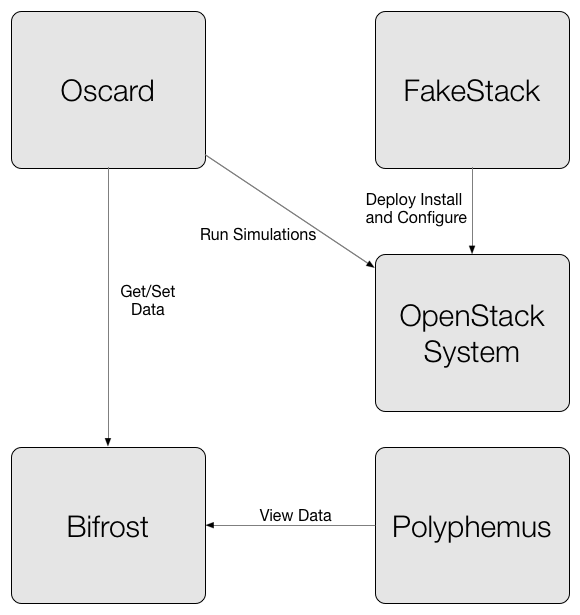
\includegraphics[width=\textwidth]{images/adock_high_arch.png}}
\label{fig:adock_high_arch}
\caption{aDock high level architecture}
\end{figure}

\subsection{Non-Functional Requirements}
\label{sub:nonfunc_req}
aDock also has very strong non-functional requirements, to give a suitable testing environment to our stakeholders. In general we take leverage of Docker and DevStack and use their biggest strength. Docker gives us i) high speeds in running containers, ii) sandboxing by construction, and iii) makes aDock cross-platform. DevStack gives us great flexibility and configurability for what concerns OpenStack services.

\paragraph{NFR1}\label{p:nfr1} \emph{Users should be able to choose which OpenStack's code version is running.} \hfill \\
Before booting the entire system the user should be able to choose if he/she wants to run OpenStack code from a precise code repository which is, in general, the better way to version and share code amongst developers. Speaking in Git\footnote{\url{http://git-scm.com/}} terms, a user could choose to run the most up to date code (which may be buggy) and so get the code from branch \code{master}, or maybe get a much more stable OpenStack version and get the code from branch \code{stable/juno}. The most interesting fact (and this is the scenario we have in our mind) is that the user could choose to fork an OpenStack service and see his/her code running nodes.

\subparagraph{Solution} All of this is achievable thanks to DevStack, which installs OpenStack services by cloning repositories from GitHub and running \code{python setup.py install}. By default, DevStack clones official OpenStack repositories from branch \code{master}, but it is possible to specify different repository URLs and branches for each of the OpenStack services by means of \code{local.conf} files.

\paragraph{NFR2}\label{p:nfr2} \emph{aDock should be lightweight.} \hfill \\
Users often need to test algorithms that, by design, target the management and/or optimization of tens of physical servers. Since we can assume that not everyone will have that amount of resources, we believe that aDock should be as light-weight as possible. It should be possible to run aDock on limited hardware, potentially even on one's personal laptop. It is under this assumption that sandboxing becomes important; indeed, the experimentation environment should not have any sort of repercussions on the user's machine; we want the user to be able to build and tear down the environment with no consequences.

\subparagraph{Solution} Docker is a virtualization system which relies on Docker containers which are much more lightweight than virtual machines\footnote{From Docker: ``Containers boot 1000x faster than virtual machines; their disk and memory footprint are also much lower; and they work on virtually all current platforms'' (see \url{https://www.docker.com/company/careers/?gh_jid=47837}).}\footnote{\url{http://devops.com/blogs/devops-toolbox/docker-vs-vms/}} \todo{are those refs authoritative?}. Docker gives us, by construction, speed and lightness.

\paragraph{NFR3}\label{p:nfr3} \emph{The experimentation environment should be highly configurable.} \hfill \\
Our primary goal with aDock is to provide a fast and easy way to create the experimentation environment. We believe that building a system which allows users to design the overall architecture of the cloud system is out of scope of this thesis, mainly because of the intrinsic high complexity and vastness of OpenStack's system itself. Up to now, as a proof of concept, we will focus on ``1 + N'' architecture, with $1$ controller node and $N$ compute nodes.

\subparagraph{Solution} The possibility to configure the system still remains in configuring OpenStack services in terms of their internal behavior. This is achieved, again, thanks to DevStack, which allows us to configure all aspects of OpenStack through its \code{local.conf} file. Each service can be configured in each of DevStack's installation phases. Each service, during installation, passes through \textbf{local}, \textbf{pre-install}, \textbf{install}, \textbf{post-config}, \textbf{extra} phases\footnote{\url{http://docs.openstack.org/developer/devstack/configuration.html\#local-conf}}. Configuring a service is as simple as adding few lines to \code{local.conf} file:

\begin{lstlisting}[title=Adding per-service configuration to DevStack's local.conf file]
... # DevStack configurations

[[post-config|\$NOVA-CONF]]
[DEFAULT]
verbose=True
logdir=/var/log/my-nova-logdir

# SCHEDULER
compute_scheduler_driver=nova.scheduler.MyMagicScheduler
# VIRT DRIVER
compute_driver=nova.virt.fake.MyAmazingFakeDriver
\end{lstlisting}


\paragraph{NFR4}\label{p:nfr4} \emph{aDock should allow users to run repeatable simulations.} \hfill \\
It is of paramount importance that users be able to compare their results with baseline approaches, as well as with related work from the state of the art. aDock should make it easy to compare an experiment's results with those of others on the same simulations.

\subparagraph{Solution} Oscard will take into account repeatability both giving the possibility to run the same simulation, at the same time, on multiple hosts, both using pseudo-randomization (see section \ref{sec:oscard}).

% --------------------------------------------------------------------------- %
% -------------------------------- FAKESTACK -------------------------------- %
% --------------------------------------------------------------------------- %

\section{FakeStack}
\label{sec:fakestack}
FakeStack\footnote{\url{https://github.com/affear/fakestack}} is the aDock module that allows the user to manage \textit{nodes}, the building blocks of an OpenStack system. Nodes are of two types: \textit{controllers} and \textit{computes}\footnote{In FakeStack, compute nodes, by default, are equipped with \code{nova.virt.fake.Fakedriver}. Thus, FakeStack compute nodes don't host a real hypervisor such as \textit{Libvirt}. Virtual machines, in FakeStack, are mere python objects. This fact, doesn't influence user's choices. A user, in fact, can equip FakeStack's compute nodes with \code{nova.virt.libvirt.driver.LibvirtDriver} as long as he/she satisfies its dependencies (this brings to editing \texttt{Dockerfile} and rebuild node's image).}. Both of them are Ubuntu-based Docker containers shipped with pre-installed software that satisfies most\footnote{main services as \textit{Nova}, \textit{Keystone}, \textit{Glance} are actually supported.} of OpenStack's services dependencies. Both controller and compute nodes are configurable by means of simple configuration files ~\ref{sub:fakestack_conf}.\\
FakeStack provides a set of scripts to handle node startup, service updating on live nodes and other features~\ref{sub:fakestack_scripts}.

\subsection{Nodes}
\label{sub:fakestack_nodes}
As already anticipated in requirement~\ref{p:nfr3}, we will focus on ``1 + N'' architectures. This architecture is characterized by $1$ controller node that handles $N$ compute nodes.\\
The main difference between a controller and a compute node is that the former contains a database (in our case, \textit{MySQL}) and a message broker (in our case, \textit{RabbitMQ}); both are compulsory for OpenStack's controller nodes.

To understand how FakeStack really works, it is useful to examine its internal structure:

\begin{figure}[H]
\centering{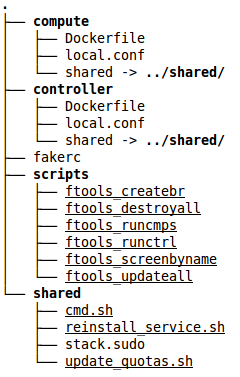
\includegraphics[height=9cm]{images/fakestack_tree.png}}
\label{fig:fakestack_tree}
\caption{FakeStack's file structure}
\end{figure}

As we can see in figure~\ref{fig:fakestack_tree}, nodes have two separated \texttt{Dockerfile}s (which makes them two different Docker containers), but they share a set of scripts (contained in the \texttt{shared} folder):

\begin{description}
	\item[cmd.sh] This is the script that will be run when the container starts (\code{docker run}). In algorithm~\ref{alg:cmd.sh} we explain its behavior in terms of pseudo-code.
	\begin{algorithm}[H]
	\caption{\texttt{cmd.sh} behavior}
	\label{alg:cmd.sh}
	% 1 is for "number any line", 0 for "no"
	\begin{algorithmic}[0]
		\If{node is \emph{controller}}
			\State set last IP in Docker bridge \Comment{assign static IP address to \emph{controller}}
		\EndIf

		\State ping 8.8.8.8 \Comment{Check internet connection}

		\If{node is \emph{controller}}
			\State start \texttt{mysql}
			\State start \texttt{rabbitmq-server}
		\EndIf

		\State \textbf{./stack.sh} \Comment{real OpenStack installation (using DevStack)}

		\State /bin/bash \Comment{let the user work on the container}
	\end{algorithmic}
	\end{algorithm}
	
	\item[reinstall\_service.sh] This script allows the user to update a service on this node specifing its name (e.g. \texttt{nova}, \texttt{glance} and so on)

	\item[update\_quotas.sh] This script allows the user to enlarge \textit{quotas} for the \textit{tenant}\footnote{\textit{Quotas} are limits on how much CPU, memory and disk space the tenant can use. \textit{Tenant} is an OpenStack concept similar to Linux groups.} in use (in our case \texttt{admin}) to a very big amount. Its usage is justified by the fact that the user will probably spawn hundreds or thousands of virtual machines on his/her OpenStack nodes, and that, normally, standard quotas will prevent him from doing so. Enlarging quotas is an easy and fast way to allow the user not to worry about how many virtual machines he owns.
\end{description}

Once a node has been built, all of the shared scripts are copied to the file-system of the node.\\
When building a container, in fact, we specify in \texttt{Dockerfile} which files have to be copied into container's file system. The files specified are copied at build-time and subsequent changes on user's file system will not result in a modification at container's file system. \textit{Data Volume}\footnote{\url{https://docs.docker.com/userguide/dockervolumes/\#data-volumes}} is a feature of Docker's that allows modifications on files to be immediately applied to container's file system. \texttt{local.conf} file \emph{is} a \textit{Data Volume}, thus it is ``bound'' to the node's file-system, in order to avoid rebuilding at each modification.

When a node is started, \texttt{cmd.sh} will run, which in turn will run DevStack's \texttt{stack.sh} (see section \ref{sec:devstack}). At that point OpenStack's installation starts.

\subsection{Scripts}
\label{sub:fakestack_scripts}
Once a user enters FakeStack's root directory he/she has to perform \code{source fakerc}. Executing this command all of the scripts contained in the \texttt{scripts} directory become available in \texttt{PATH}. The prefix \texttt{ftools\_} is added to avoid conflicts in names.\\
Scripts for running and updating nodes leverage Linux screens\footnote{\url{http://linux.die.net/man/1/screen}}. Screens is a powerful tool to run detached shells from within another shell. This feature gives lots of advantages both in terms of ease of use and in running long running jobs via SSH.\\
All of aDock processing is confined into two different screens, \texttt{running} and \texttt{updating}. Thanks to this, the user will not have to open lots of shells, but focus on using only one; keeping it clean from computation and reattaching to aDock screens when needed. If the user wants to run a long running task (e.g. a very long simulation or lots of different, small simulations) on a remote server via SSH, he will not need to keep the SSH session open and wait for simulations to end; the screen session, in fact, will stay open (and so the processes within it, running) independently from the SSH connection. 

We now list and describe the scripts contained in the \texttt{scripts} directory.
\begin{description}
	\item[createbr] Input: bridge name. Creates a bridge with CIDR $42.42.0.0/24$; it takes the name passed as first argument by the user. This bridge is intended to be used by Docker, setting the option \code{-b <bridge\_name>} into \texttt{/etc/default/docker}. Run this script before starting the system or editing the IP configuration in \texttt{cmd.sh}. In fact, \texttt{cmd.sh} will set the controller's IP to the last IP available in that precise network ($42.42.255.254$). After running this script, Docker service has to be restarted.
	\item[destroyall] Stops and destroys all OpenStack nodes.
	\item[runctrl] Runs one controller node on a new window in screen \texttt{running}.
	\item[runcmps] Input: \texttt{N}. Starts \texttt{N} compute nodes concurrently\footnote{They are started as Docker daemons (\code{-d} option in Docker).}. A new window (\texttt{cmps}) in screen \texttt{running} is created asking for operation confirmation. Once the opration is confirmed, nodes are started and a new window (\texttt{samplecmp}), attached to one of the compute nodes, is opened to show the user a sample node behavior and progress in OpenStack installation.
	\item[screenbyname] Input: screen name. Reattachs to the screen named as given by the user, if it exists.
	\item[updateall] Input: service name. Updates the service given by the user on all OpenStack nodes. All of the processing is performed into screen \texttt{updating}.
\end{description}

We will now list and describe the scripts ``sourced'' by \texttt{fakerc} (\texttt{ftools\_} convention is always maintained).
\begin{description}
	\item[runcmp] Alias for \code{ftools\_runcmps 1}.
	\item[build] Input: \texttt{ctrl} or \texttt{cmp}. This script builds the node; regenerating it from a pure Ubuntu image. It is necessary to run this script only in case some of the files (apart from \texttt{local.conf}) have been modified.
	\item[attach] Input: container ID. Attaches to a Docker container. Alias for \code{docker attach <container\_id>}.
\end{description}

\subsection{Configuration}
\label{sub:fakestack_conf}
\todo{repair listings placement!}

Fakestack leverages the powerful configurable options of DevStack. Modifying \texttt{local.conf} files before starting a node, it is possible to change the enabled services (see listing~\ref{lst:enabled_services}) and their internal configuration (see listing~\ref{lst:driver_conf}). Every service is configurable in each of its installation \textit{phases}, which are, for DevStack, \textbf{local}, \textbf{pre-install}, \textbf{install}, \textbf{post-config}, \textbf{extra}\footnote{For more information see \url{http://docs.openstack.org/developer/devstack/configuration.html\#local-conf}}. Configuring it is as simple as adding a \code{[[ <phase> | <config-file-name> ]]} line (e.g. \code{[[post-config|\$GLANCE\_CONF]]}) to \texttt{local.conf} file and add configuration options below.\\
Most important, it is possible to choose a different Git repository and Git branch for each of OpenStack's services enabled (see listing~\ref{lst:change_repo}). DevStack, in fact, install services \textit{cloning} those repositories and running \code{python setup.py install}\footnote{\label{note:pypi}It is the standard way to install \textit{PyPI} packages. More information can be found at \url{https://wiki.python.org/moin/CheeseShopTutorial}}.\\
Thanks to this important piece of configuration, a user can \textit{fork} an OpenStack project; develop its code and use its new forked repository URL in DevStack's configuration.\\
In listing~\ref{lst:localconf_ex} we show a possible complete example of \texttt{local.conf} file for a compute node.

\begin{lstlisting}[floatplacement=H, caption={Choose OpenStack's enabled services}, label={lst:enabled_services}, numbers=none]
... # Other configuration options

# Enables:
# - Nova Compute
# - Nova API
# - Nova Network
ENABLED_SERVICES=n-cpu,n-api,n-net

... # Other configuration options
\end{lstlisting}

\begin{lstlisting}[floatplacement=H, caption={Internal configuration of Nova}, label={lst:driver_conf}, numbers=none]
... # Other configuration options

[[post-config|$NOVA_CONF]]
[DEFAULT]
compute_driver=nova.virt.fake.MyFakeDriver

... # Other configuration options
\end{lstlisting}

\begin{lstlisting}[floatplacement=H, caption={Change repository URL}, label={lst:change_repo}, numbers=none]
... # Other configuration options

NOVA_REPO=https://github.com/me/nova.git
NOVA_BRANCH=my-branch

... # Other configuration options
\end{lstlisting}

\begin{lstlisting}[floatplacement=H, caption={Complete \texttt{local.conf} example for compute node}, label={lst:localconf_ex}]
[[local|localrc]]
FLAT_INTERFACE=eth0
MULTI_HOST=1
LOGFILE=/opt/stack/logs/stack.sh.log
SCREEN_LOGDIR=$DEST/logs/screen

NOVA_REPO=https://github.com/me/nova.git
NOVA_BRANCH=my-branch

DATABASE_TYPE=mysql

ADMIN_PASSWORD=pwstack
MYSQL_PASSWORD=pwstack
RABBIT_PASSWORD=pwstack
SERVICE_PASSWORD=pwstack
SERVICE_TOKEN=tokenstack

SERVICE_HOST=controller
MYSQL_HOST=controller
RABBIT_HOST=controller

NOVA_VNC_ENABLED=False
VIRT_DRIVER=fake

ENABLED_SERVICES=n-cpu,n-api,n-net

[[post-config|$NOVA_CONF]]
[DEFAULT]
compute_driver=nova.virt.fake.MyFakeDriver
\end{lstlisting}

\subsection{Example}
\label{sub:fakestack_ex}
In this section we provide an example on how to use FakeStack in a pseudo-code fashion.\\
Procedure~\ref{alg:example} is comprehensive of real bash commands, aDock's commands and standard input to handle Linux screens. It refers to a user that wants to launch a ``1 + 5'' architecture from scratch. In this case we suppose that the user will start a ``vanilla'' OpenStack version, and so he/she doesn't need to modify any configuration files.

\begin{algorithm}[H]
\caption{Launching a ``1 + 5'' architecture with aDock}
\label{alg:example}
\begin{algorithmic}[0]
	\State \texttt{git clone https://github.com/affear/fakestack}
	\State \texttt{cd fakestack}
	\State \texttt{source fakerc} \Comment{all aDock commands are now available}
	\State \texttt{ftools\_createbr docbr} \Comment{``docbr'' is the name of the new bridge}
	\State \texttt{sudo nano /etc/default/docker} \Comment{adding \code{-b docbr} option to Docker's configuration}
	\State \texttt{sudo service docker restart}
	\State % blank line
	\State \texttt{ftools\_runctrl}
	\State \Comment{waiting for controller to finish installation}
	\State \texttt{ftools\_runcmps $5$}
	\State \texttt{screen -R} \Comment{attaching to the only screen active (\texttt{running}). Window is \texttt{ctrl}}
	\State \emph{\texttt{CTRL+A N}} \Comment{window is now \texttt{cmps}}
	\State
	\State \emph{enter \texttt{y} to confirm that a controller node is up and we want to start compute nodes}
	\State
	\State \Comment{wait for compute nodes to finish}
	\State \emph{\texttt{CTRL+A P} for two times} \Comment{\texttt{ctrl} window}
	\State \texttt{source openrc admin admin}
	\State \texttt{nova service-list} \Comment{$5$ compute nodes should be shown}
	\State \texttt{nova boot --image cirros --flavor 1 samplevm} \Comment{Spawns a new virtual machine}
	\State \ldots
	\State \ldots \Comment{enjoy your OpenStack environment}
\end{algorithmic}
\end{algorithm}

% --------------------------------------------------------------------------- %
% ---------------------------------- OSCARD --------------------------------- %
% --------------------------------------------------------------------------- %

\section{Oscard}
\label{sec:oscard}
Oscard\footnote{\url{https://github.com/affear/oscard}} is the aDock module that takes care of running simulations against one or more OpenStack systems and collecting their data outputs. Oscard has two main components, a server and a client (see \ref{sub:oscard_internals}). The two components don't need to be used on the same machine. This is why Oscard's dockerized version only runs the server part and waits for requests from the client.

The client part is the one that defines simulation running behavior. The user is supposed to use the client to actually start simulations by means of an executable file (\code{\$ ./bin/run\_sim}).

The server part is the \textit{Proxy}, it literally waits for client requests and forwards them to OpenStack's controller node and stores simulation's outputs into Bifrost (see section \ref{sub:bifrost}).

Oscard is completely configurable from the \texttt{oscard.conf} file.

\subsection{Modules}
\label{sub:oscard_modules}
Oscard is composed of few modules (see figure \ref{fig:oscard_tree}); in this section we will explain in detail what each of them is up to.

\begin{figure}[H]
\centering{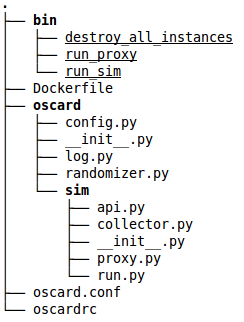
\includegraphics[height=8cm]{images/oscard_tree.png}}
\label{fig:oscard_tree}
\caption{Oscard's file structure}
\end{figure}

\begin{description}
	\item[oscard.sim.api] This module contains the APIs to interact with OpenStack's Nova.
	It contains two classes, \code{NovaAPI} and \code{FakeAPI}. \code{NovaAPI} provides the methods necessary to perform basic operations on Nova using OpenStack's official python clients: \code{keystoneclient.v2\_0} and \code{novaclient.v1\_1}.

		\begin{itemize}
			\item \code{init}: resets APIs random seed. If the option \texttt{random\_seed} has been modified in \texttt{oscard.conf}, the new seed will be reloaded as well.
			\item \code{architecture}: Returns the system's architecture in terms of compute nodes and their resources (vCPUs, memory and disk).
			\item \code{active\_services}: Returns active service and their number. For instance, if there are $10$ compute nodes, it is very common to have $10$ \texttt{nova-compute} services up. In this case, only one \texttt{nova-compute} service with count $10$ will be returned.
			\item \code{snapshot}: Returns a snapshot of the system. The snapshot contains data about each compute node in use (a node which is hosting virtual machines), such as resources in use, and aggregate data about all active nodes (averages of resources usage). 
			\item \code{create}: Spawns an instance of random flavor and returns its ID.
			\item \code{resize}: Resizes a random active instance to a random flavor (different from its actual one) and returns its ID.
			\item \code{destroy}: Deletes a random instance.
		\end{itemize}

	\code{FakeAPI} class, mimics \code{NovaAPI}'s behavior but it doesn't involve an OpenStack controller. It was developed only for testing purpose.
	\item[oscard.sim.collector] This module exposes the \code{BifrostAPI} class; this API gives a way to interact with the Firebase backend for data storage. An instance of \code{BifrostAPI} is obtained in the \code{oscard.sim.run} module, and is used to store the data obtained during the simulation.
	\item[oscard.sim.proxy] This module contains the API to communicate with the proxy (\code{ProxyAPI}). The class basically mirrors the methods contained in \code{oscard.sim.api.NovaAPI}. A \code{NovaAPI} object is obtained when the module is started, to which calls are \textit{delegated}. It is this module that, if run from module \code{\_\_main\_\_}, starts a WSGI server (powered by Bottle\footnote{\url{http://bottlepy.org/docs/dev/index.html}}) and waits for GET and POST requests.
	\item[oscard.randomizer] This module is a wrapper for python's \code{random} module. It provides \code{get\_randomizer} function which returns a new \code{random.Random} object initialized with the same seed as specified in \texttt{oscard.conf}.
\end{description}

\subsection{Oscard Internals}
\label{sub:oscard_internals}
\newcommand{\osconf}[1]{\footnote{In \texttt{oscard.conf}: \texttt{#1}}}

In this section we will describe how Oscard internal works, and how it can be configured. We will also clarify how we use pseudo-randomness within simulations.

Each randomized decision in Oscard is taken using a randomizer obtained through \code{oscard.randomizer.get\_randomizer}. Each time we get a randomizer, it is initialized with a seed taken from a configuration file\osconf{random\_seed} or, in case one is not specified, directly from Bifrost's last simulation ID (The seed used is equivalent to the simulation ID that the user wants to execute). It is for this reason that every randomized decision can be repeated simply setting the seed in the configuration file.

Every simulation is composed of a precise number of commands\osconf{no\_t} run in sequence. Each command is executed at a precise step which is a discrete instant in time. Currently available commands are \textit{create}, \textit{resize}, \textit{destroy} and \textit{NOP}. The first three commands are clear in their intent; the last one, i.e. the \textit{NOP} command, is a ``no operation'' command. It is meant to make simulations more realistic in the sense that, in reality, it is impossible that at each time instant the system is asked to perform a CRD\footnote{Create Resize Destroy} operation. \textit{NOP} operation simulates the fact that the system could be idle (in term of requests from users) in some moments. ``No operation''s allow us to change operation \textit{density} along time.

At each step, Oscard chooses a command at random and executes it. Commands can have different weights\osconf{<command-name>\_w} that influence their probability to be chosen. Each command is executed \textit{when and only when} the command before has been completed (either successfully or not); thus, the state of the machine that is interested in the operation, can be one of \texttt{ACTIVE} or \texttt{ERROR}\footnote{Two of possible instance states in OpenStack. See \url{http://docs.openstack.org/developer/nova/devref/vmstates.html}.}. Because of this reason, and because Oscard is single-threaded, we can say that Oscard's simulations are run \textit{serially}. This fact is important, because in conjunction with pseudo-randomness, it ensures \textit{simulation repeatability}. At least, for what concerns Oscard itself: the system, in fact, is built to run repeatable simulations, but we cannot guarantee that the OpenStack system will always take the same decisions. Thus, two simulation outputs could be different even if simulations are, for Oscard, the same one.

As already said, Oscard is composed of two parts, the server and the client one. Oscard's proxy (the server part) can be run both as a Docker container or running \code{./bin/run\_proxy} from a shell\footnote{Dockerized version is recommended, because it allows the user not to install all Oscard's dependencies before running}. Oscard, as FakeStack, has a source file called \texttt{oscardrc}. Once the user runs \code{source oscardrc}, \code{run\_oscard} script is available in \texttt{PATH}, this script can be used to start Oscard's container.

Oscard is highly configurable, but it is important to note that each option has a default value (see \url{https://github.com/affear/oscard/blob/master/oscard.sample.conf}). So, it is not needed to configure each Oscard option before starting it. Some options are relevant only for server, others for client and some for both of them. We list their meaning and split them between the two Oscard components to better understand their working.

The server part can be configured in terms of:
\begin{itemize}
	\item \texttt{proxy\_port}: sets the port on which Oscard's proxy will listen on.
	\item \texttt{os\_username}, \texttt{os\_tenant}, \texttt{os\_password}: access credentials for the user used in OpenStack.
	\item \texttt{fake}: if set to \code{True}, \code{FakeAPI} will be used.
	\item \texttt{ctrl\_host}: the IP of the docker container running controller node.
	\item \texttt{fb\_backend}: it's the Firebase backend URL.
	\item \texttt{random\_seed}: the seed that \code{NovaAPI} will use to choose random instances and random flavors. Set this parameter to the ID of the simulation that needs to be run.
\end{itemize}

The client part can be configured in terms of:
\begin{itemize}
	\item \texttt{fb\_backend}: as above.
	\item \texttt{random\_seed}: as above.
	\item \texttt{no\_t}: the number of steps for the simulation.
	\item \texttt{create\_w}, \texttt{resize\_w}, \texttt{delete\_w}, \texttt{nop\_w}: weights for commands.
	\item \texttt{proxy\_hosts}: the URLs for the proxies on which the simulation will be run concurrently (e.g. \texttt{host1.example.com:3000,host2.example.com:80}). Oscard, in fact, can run the same simulation concurrently on more than one host (if real-time comparisons are needed).
\end{itemize}

As an example of Oscard functioning, we show in figure~\ref{fig:oscard_functioning}, by means of a sequence diagram, the workflow of a \texttt{create} operation. 

\todo{sequence diagram of create op}

% sequence diagram
\begin{figure}[H]
\centering{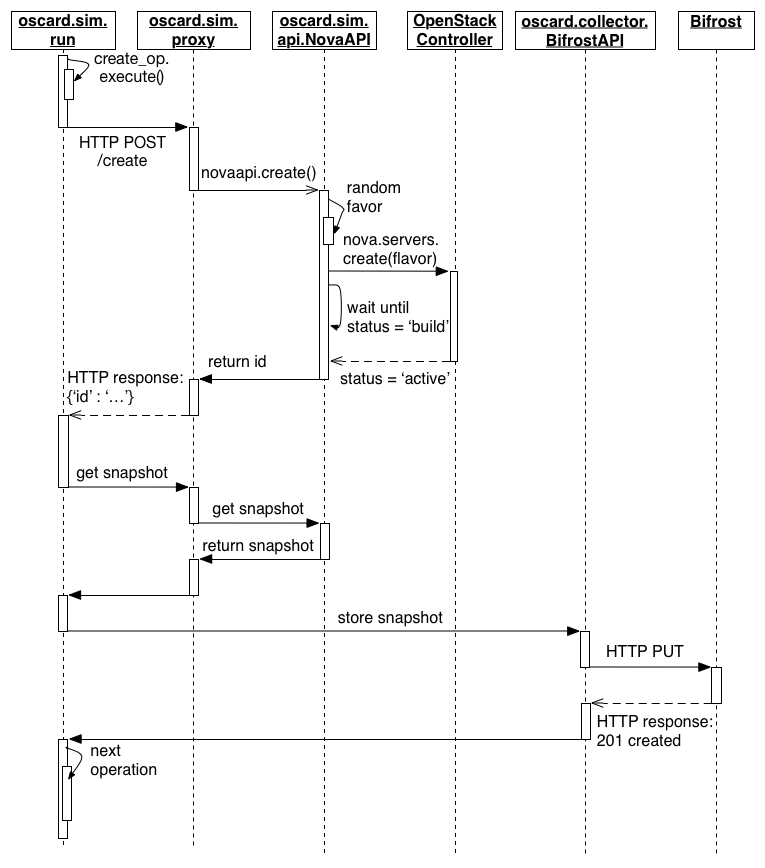
\includegraphics[width=\textwidth]{images/create_seq.png}}
\label{fig:oscard_functioning}
\caption{Workflow for a \texttt{create} operation}
\end{figure}

% --------------------------------------------------------------------------- %
% --------------------------- BIFROST + POLYPHEMUS -------------------------- %
% --------------------------------------------------------------------------- %

\section{Other Components}
\label{sec:others}
The last two components of aDock take care of its database and view. These two roles are covered respectively by Bifrost and Polyphemus.

\subsection{Bifrost}
\label{sub:bifrost}
Bifrost\footnote{\url{https://bifrost.firebaseio.com/}} is the name for the Firebase application delegated to store simulation data output. Firebase uses a non-relational JSON database. The whole aDock database is thus a JSON structure that is exportable in a \texttt{.json} file. Firebase provides a JavaScript and a python SDK and it natively supports real-time notifications on data change (only for JavaScript SDK). We decided to use this backend type because of its SDKs; for the portability of \texttt{.json} format; for the advantages of dealing with a non-relational database when data is very mutable (especially while developing); because performance is not needed in our case and because of its cloud nature. It is important that Firebase, by design, doesn't offer a great support for concurrent calls\footnote{\url{https://www.firebase.com/docs/web/guide/saving-data.html\#section-transactions}}, so, our simulations \textit{cannot} run concurrently\footnote{The same simulation can be run concurrently on more hosts, but two simulations cannot be run concurrently on different hosts.}.

Firebase offers a good dashboard (see \ref{fig:firebase_dash}) that updates in real-time (if the amount of data is not too big) and allows the user to perform CRUD\footnote{Create Read Update Delete} operations on data. 

\begin{figure}[H]
\centering{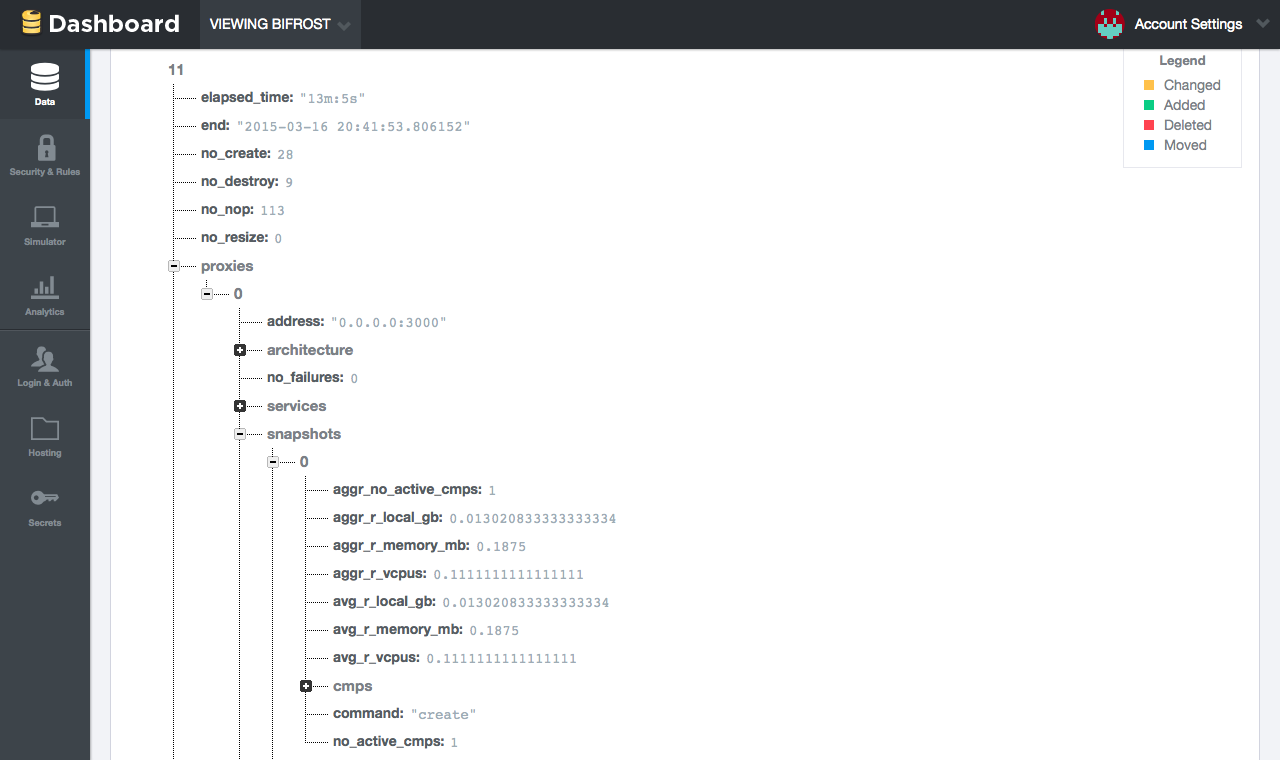
\includegraphics[width=\textwidth]{images/firebase_dash.png}}
\label{fig:firebase_dash}
\caption{Firebase Dashboard}
\end{figure}

\subsection{Polyphemus}
\label{sub:polyphemus}
Polyphems\footnote{\url{https://github.com/affear/polyphemus}} is the Polymer\footnote{\url{https://www.polymer-project.org/0.5/}}-powered view of aDock. It can be run in a Docker container or not\footnote{Dockerized version is recommended, because it allows the user not to install all Polyphemus' dependencies such as \texttt{NodeJS} before running}. Its aim is to show data to the user in a friendly way. Polyphemus shows each simulation snapshot in terms of overall average of resources usage\footnote{The average of the percentage of vCPUs, memory and disk used calculated on all active compute nodes (nodes that are hosting at least one instance).} through line charts and percentage of resources usage\footnote{The percentage of vCPUs, memory and disk.} for each compute node through bar charts. A tool-bar representing data aggregates\footnote{The average of all averages of resources usage calculated on the number of simulation steps executed.} for each host is always visible on the top. It shows charts for each of the hosts on which the current simulation is running, giving the possibility to make comparisons intuitively. Moreover it includes more information such as the architecture of each OpenStack system running on each host; active services and simulation progress.

Every information displayed by Polyphemus is updated in \textit{real-time}. In figure \ref{fig:poly}, we provide a sample screen shot of Polyphemus. 

\begin{figure}[H]
\centering{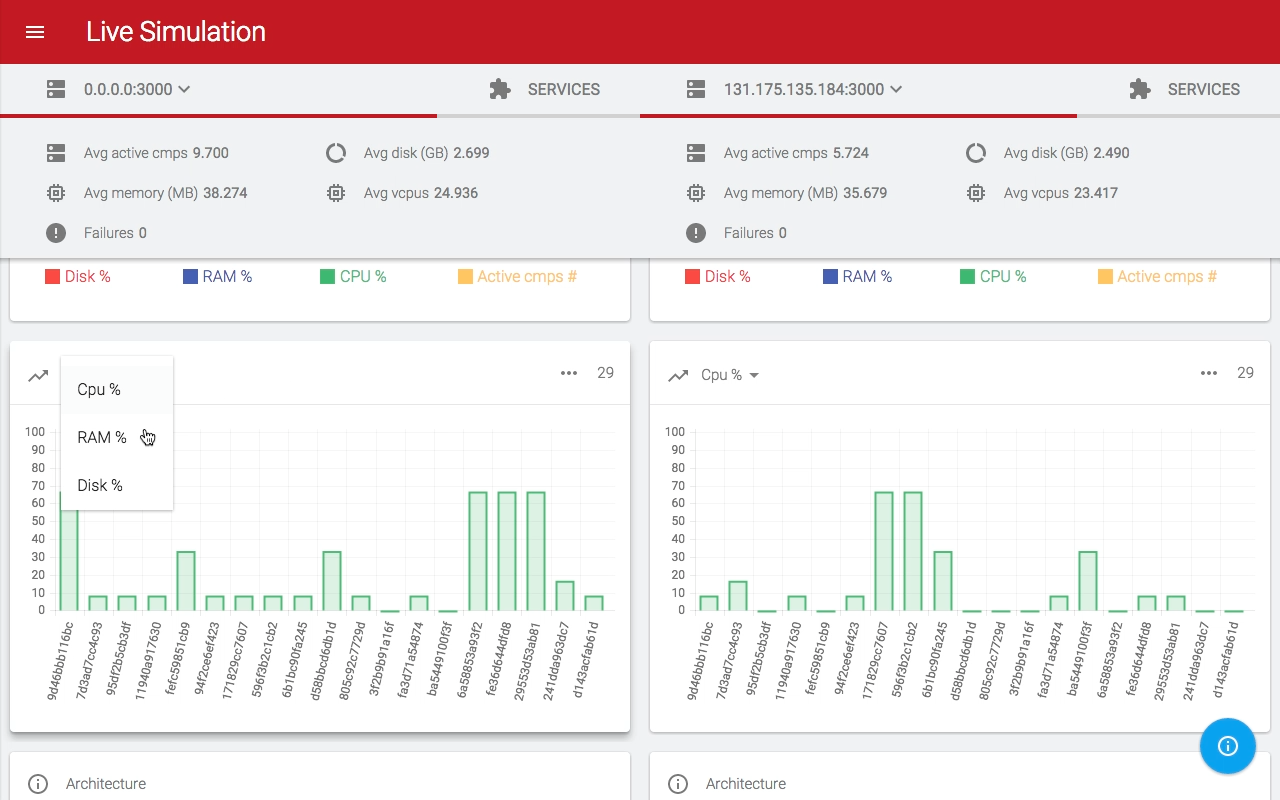
\includegraphics[width=\textwidth]{images/poly.png}}
\label{fig:poly}
\caption{Screenshot of Polyphemus}
\end{figure}

\section{aDock's Architecture}
\label{sec:adock_arch}
aDock is a modular system, where each component is run in its dockerized version\footnote{Apart from Bifrost.}. In figure \ref{fig:adock_arch}, a sample aDock architecture is shown.

The simulation is started from a normal laptop using Oscard. Oscard client contacts Oscard proxies on each of the hosts (specified in \texttt{proxy\_hosts}) using the endpoints exposed, each endpoint identifies a different command to be executed. For each host, Oscard proxy uses \code{NovaAPI} to ``send'' the command to controller node (whose IP is specified in \texttt{ctrl\_host}) which, in turn, will handle it. For each host and at each step, the proxy collects data from the controller using \code{NovaAPI} methods and stores it into Bifrost using \code{BifrostAPI}. Data is available and can be consulted connecting to Polyphemus\footnote{Polyphemus container can be started everywhere, not only on one of the hosts.} using a web browser on user's laptop.  

\begin{figure}[H]
\centering{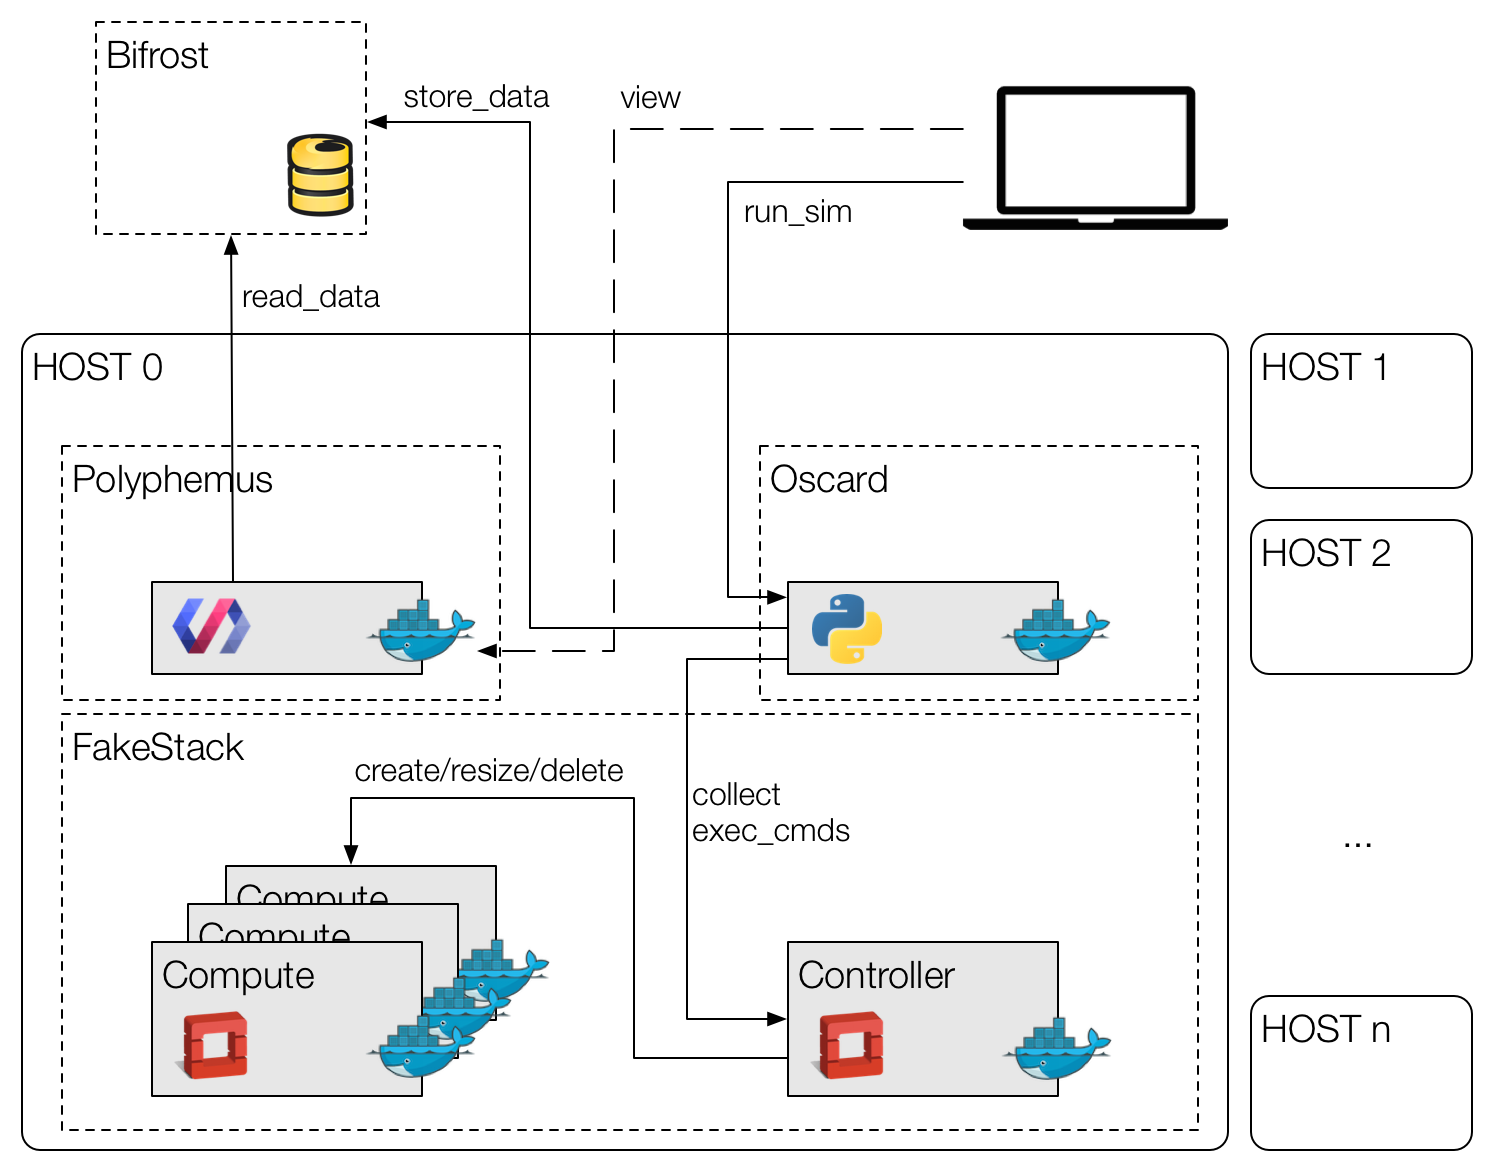
\includegraphics[width=\textwidth]{images/adock_arch.png}}
\label{fig:adock_arch}
\caption{aDock architecture}
\end{figure}